\documentclass[12pt]{article}
%--------------------   start of the 'preamble'
%
\usepackage{graphicx,amssymb,amstext,amsmath,color}
\usepackage[margin=2cm]{geometry}
\usepackage{abstract}
\usepackage{setspace}
\usepackage[footnotesize,bf]{caption}

% TABLE
\usepackage{multicol,hhline,colortbl,multirow}
\usepackage{braket}
\usepackage{siunitx}
\usepackage{hyperref}
\usepackage{authblk}
\usepackage{siunitx}
\usepackage{adjustbox}
\usepackage{mathrsfs}
%%\usepackage[sort&compress]{natbib}
%%\bibpunct{(}{)}{,}{a}{, }{;}
%
\usepackage[sort&compress]{natbib}
\bibpunct{[}{]}{,}{s}{}{;}


\definecolor{gray}{gray}{0.8}
\def\mobunits{\square\centi\meter\per\volt\per\second}
\def\gcm{\gram\per\cubic\centi\meter}
\def\ccg{\cellcolor{gray}}

\renewcommand{\labelitemii}{$\circ$}
\renewcommand{\bibname}{References}


\title{MorphCT Results - Outstanding Questions}
\author{Matthew Jones}
\date{\today}

\begin{document}
\maketitle

\section{Summary}

This document is an addendum to both the Voronoi Neighbour Analysis and the Neat P3HT results to consider the differences between the OrigFG and the NewFG results.
The centre-of-mass deviations from the CG morphology to the final chromophore positions after fine-graining are all located within 5~\AA, with the majority of chromophores around 2~\AA~away from their initial positions.

I then consider why the $T = 2.25$ system has such a low mobility.
The fit quality is bad due to a poorly connected network using the Voronoi analysis, leading to a saturating MSD and carriers not moving sufficiently far during the simulations.
This could be rectified by considering additional structurally decorrelated frames to provide error bars on the mobility.

\subsection{CoM Deviations}

\begin{figure}[h!]\centering
	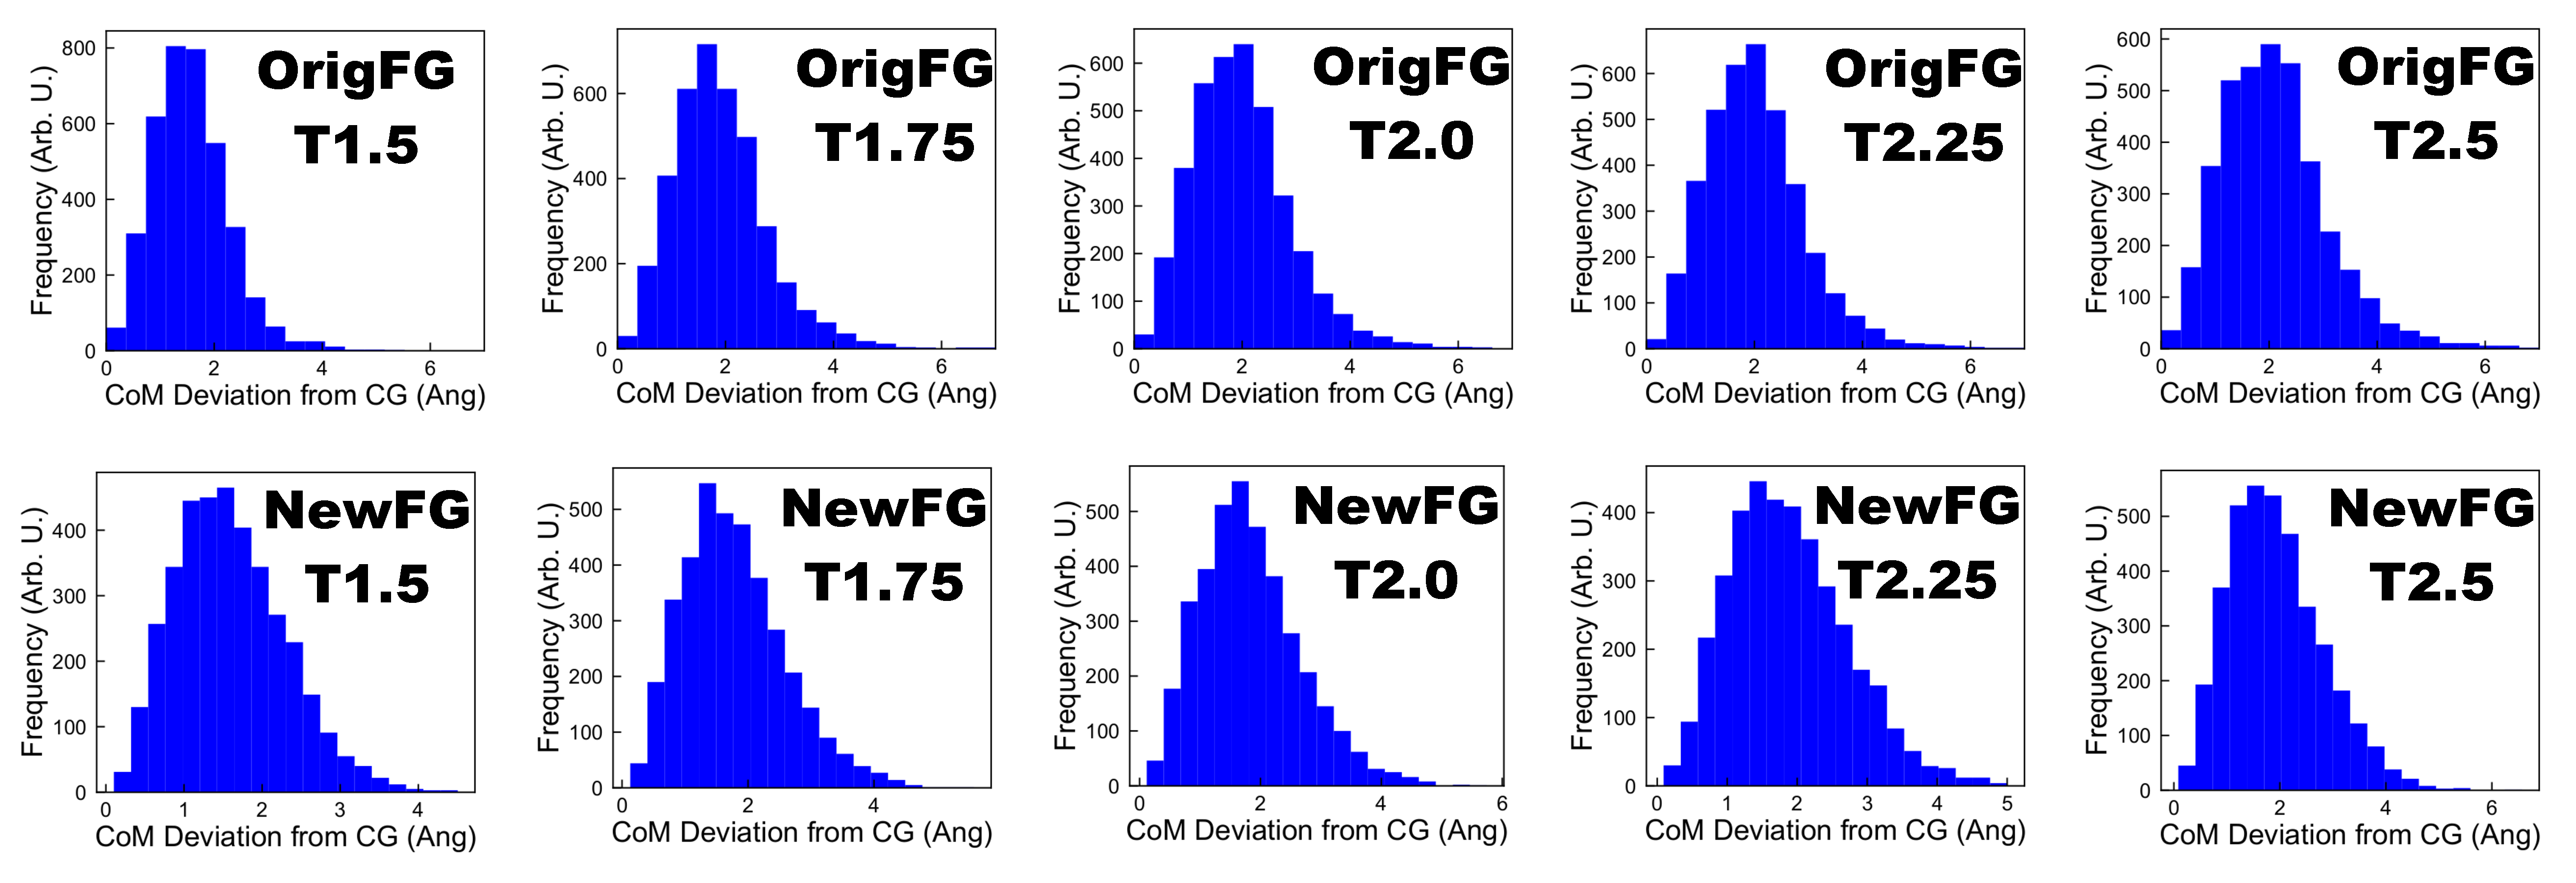
\includegraphics[width=\textwidth]{Figures/CoMDeviation.pdf}
    \caption{The distribution of physical deviations between the coarse-grained bead centre of mass describing the chromophore from the input and the resultant centre of mass of the chromophore after fine-graining.}
	\label{fig:Deviation}
\end{figure}

\clearpage

\subsection{Why does the origFG-T2.25 have such a slow mobility compared to origFG-T2.0 and origFG-2.5?}


Recall the mobility curve for the origFG systems using the Voronoi analysis:


\begin{figure}[h!]\centering
	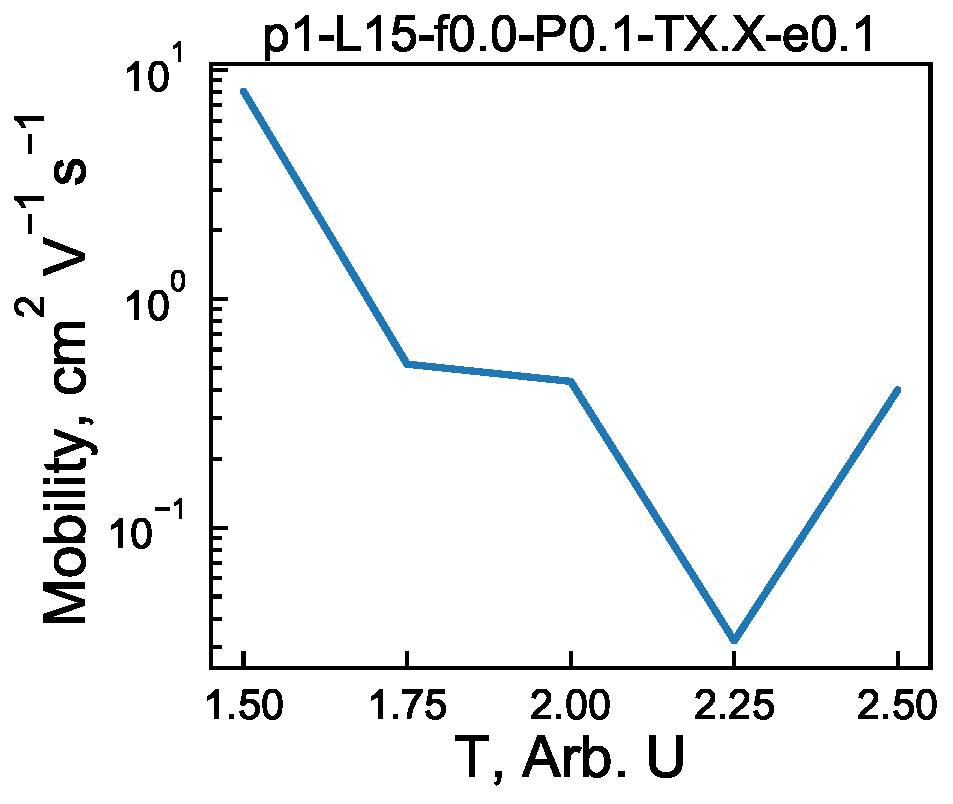
\includegraphics[width=0.6\textwidth]{Figures/origFGTempMob.pdf}
    \caption{The mobility curve for the systems with different temperature statepoints, all using the original fine-graining results.}
	\label{fig:Mob}
\end{figure}


Why does the $T = 2.25$ system have such a low mobility compared to the other disordered morphologies?
The following graphs show all of the analysis data we have for the morphologies with statepoints $2.0 \leq T < 2.5$.

\begin{figure}[hb]\centering
	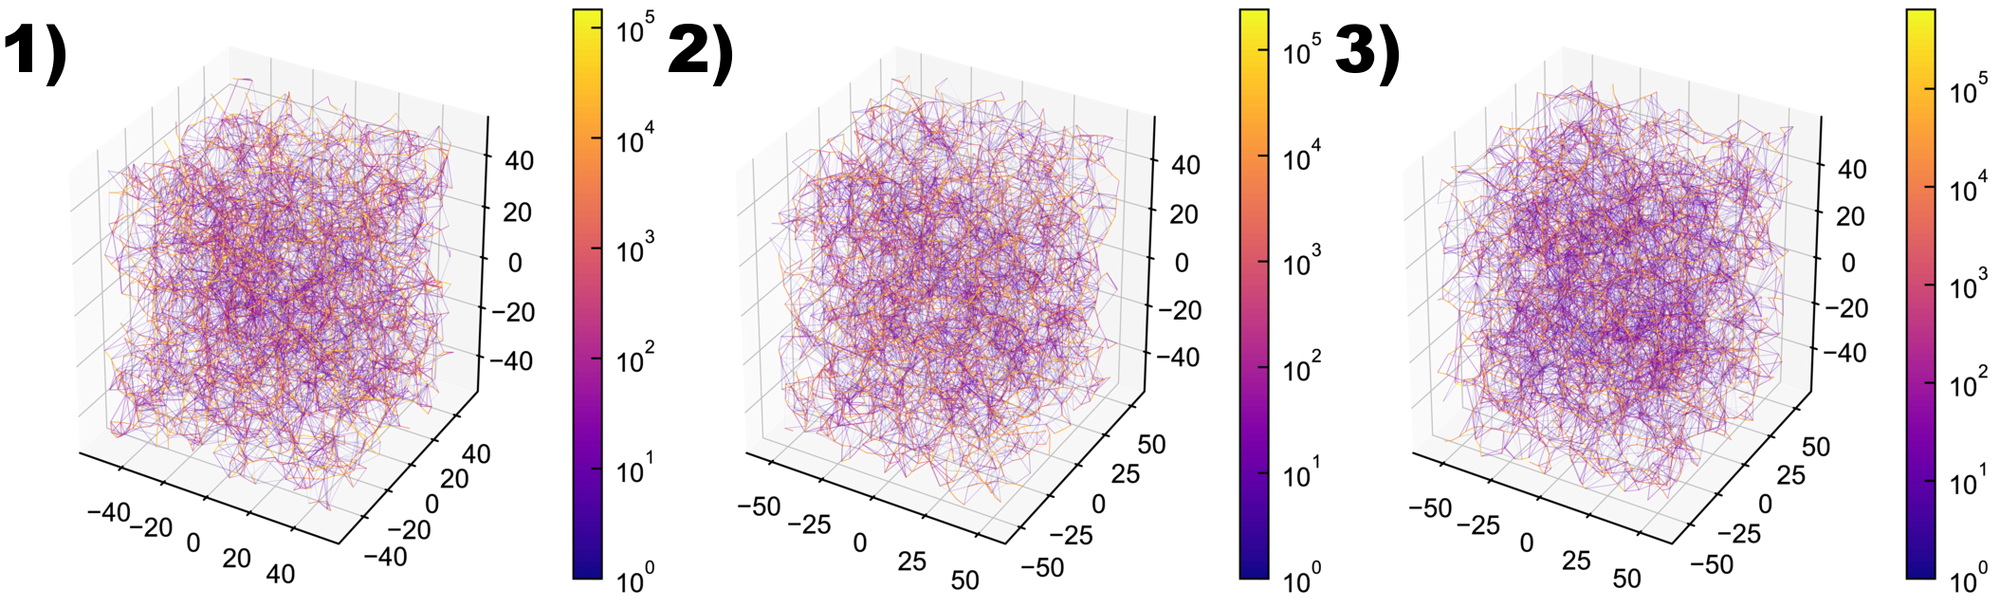
\includegraphics[width=\textwidth]{Figures/networks.png}
    \caption{The 3D Network graphs for 1) \textbf{origFG-p1-L15-f0.0-P0.1-T2.0-e0.5}, 2) \textbf{origFG-p1-L15-f0.0-P0.1-T2.25-e0.5}, 3) \textbf{origFG-p1-L15-f0.0-P0.1-T2.5-e0.5}.}
	\label{fig:net}
\end{figure}

\begin{figure}[p]\centering
	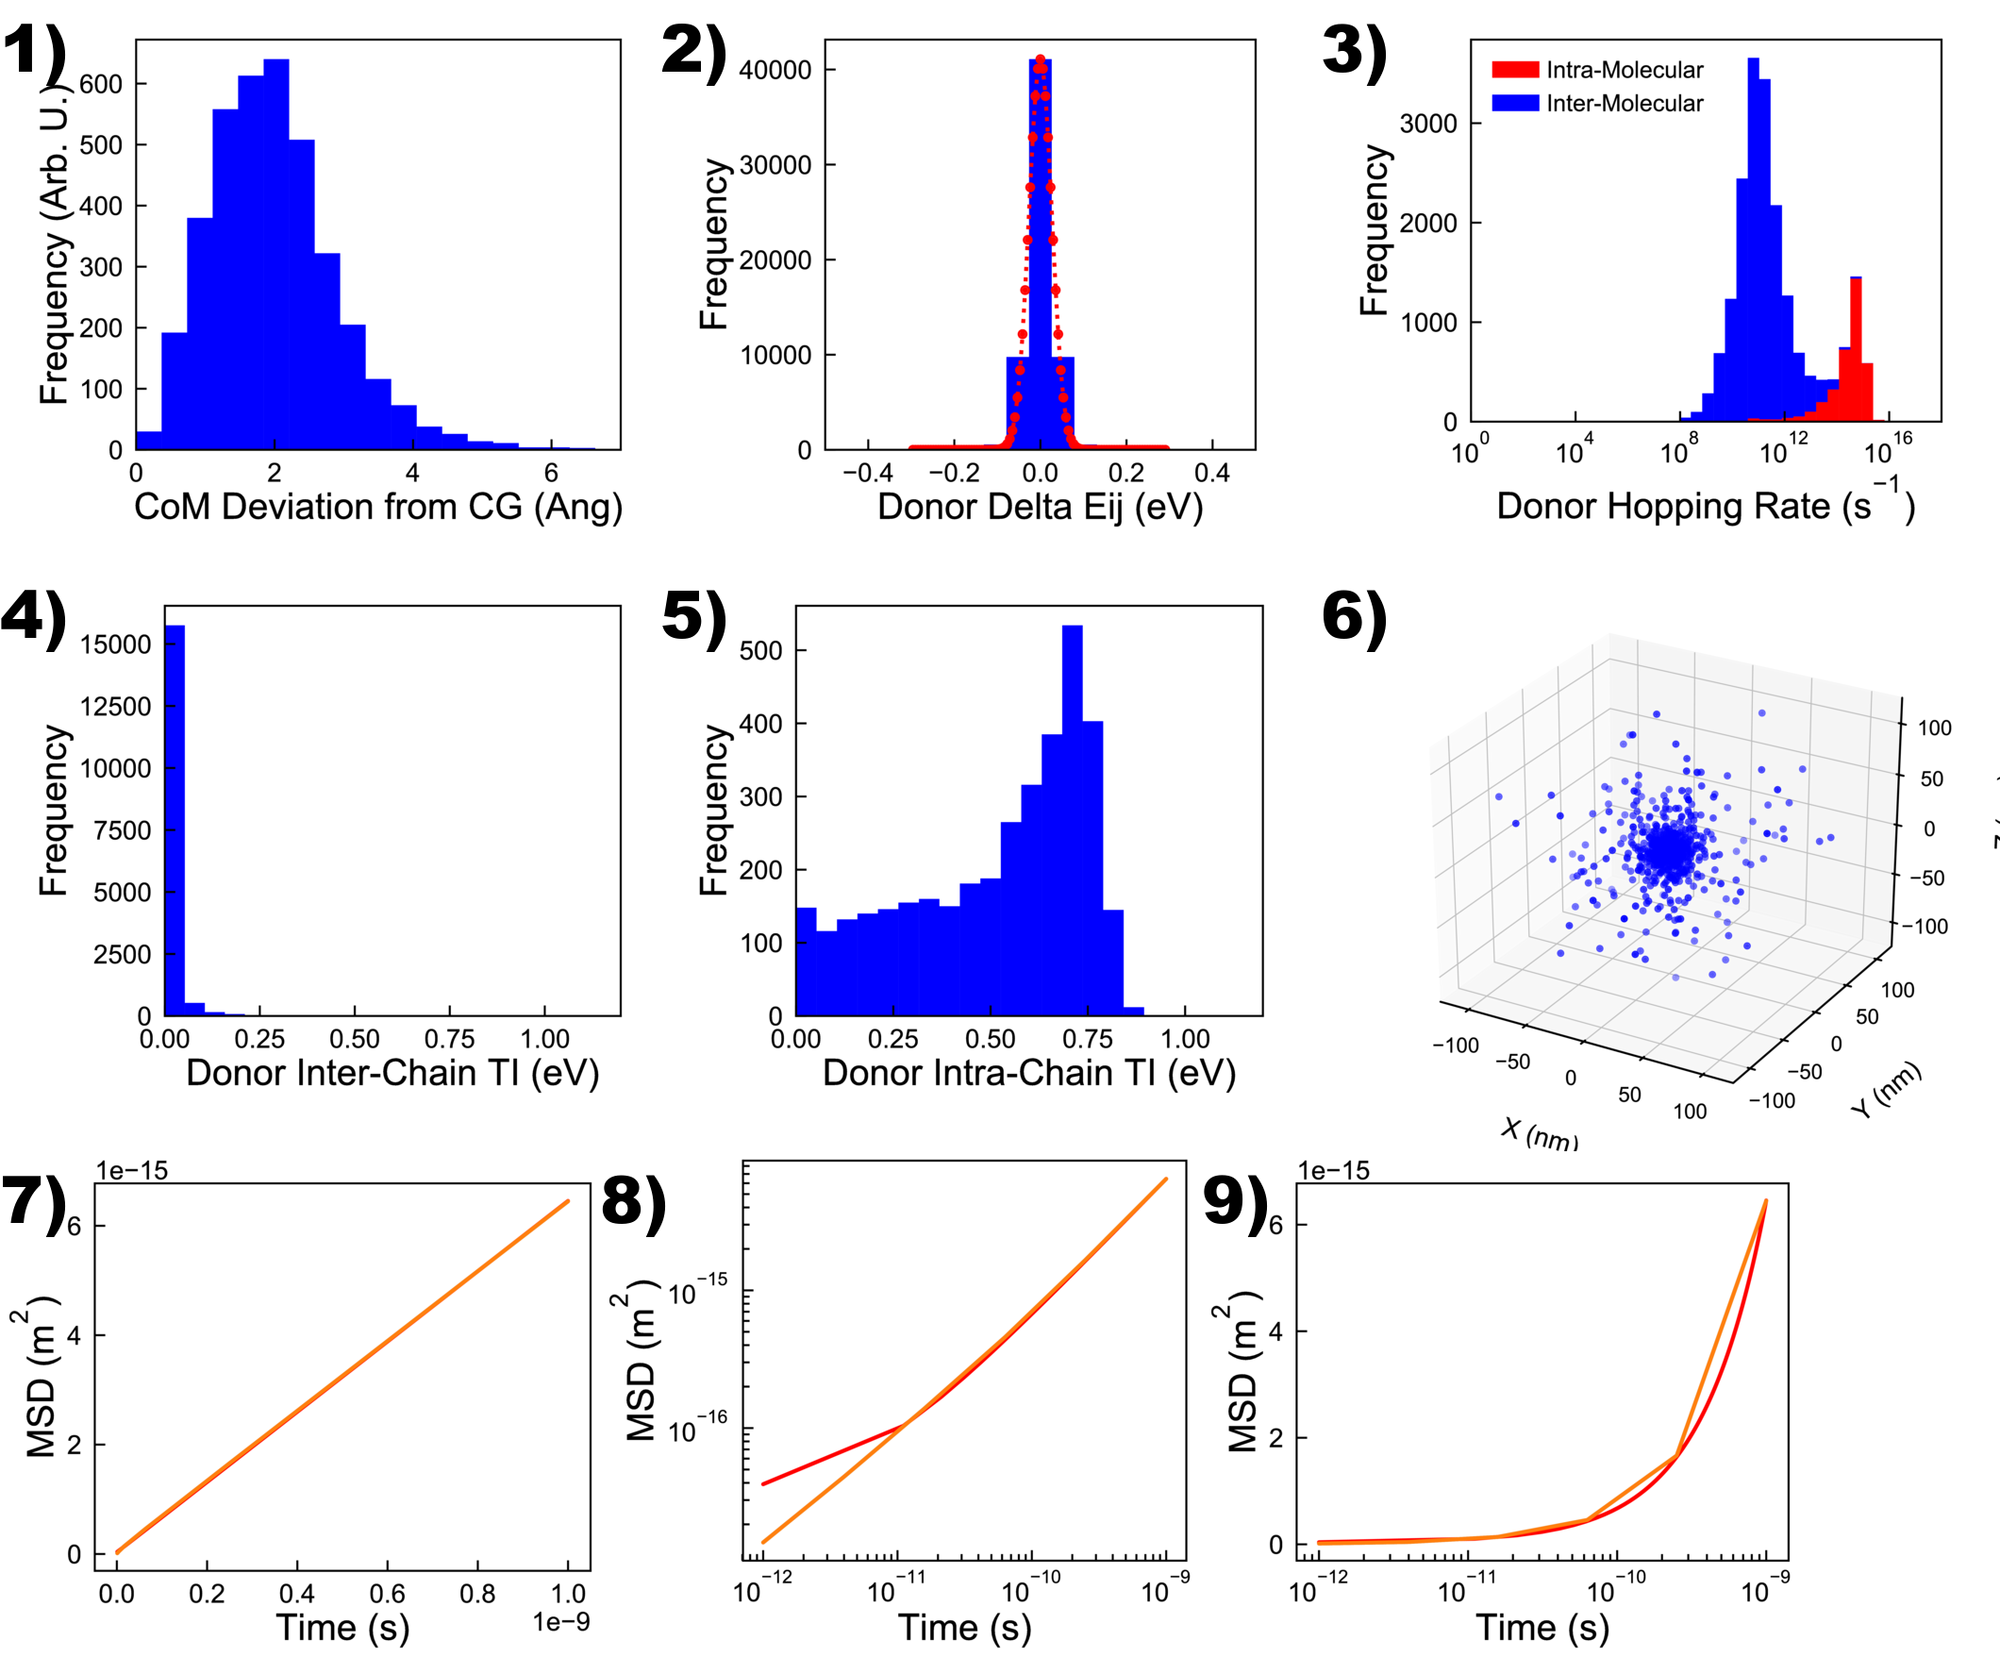
\includegraphics[width=\textwidth]{Figures/T2_0.png}
    \caption{The plots for \textbf{origFG-p1-L15-f0.0-P0.1-T2.0-e0.5}. Plots are as follows: 1) Separation between the CG and fine-grained chromophore CoM, 2) HOMO DoS for chromophores, 3) Hopping rate distribution, 4) Inter-molecular TIs (zeros removed), 5) Intra-molecular TIs (zeros removed), 6) Carrier endpoints after KMC simulation, 7) MSD (Linear scale), 8) MSD (log scale), 9) MSD (semi-log scale)}
	\label{fig:T2.0}
\end{figure}

\begin{figure}[p]\centering
	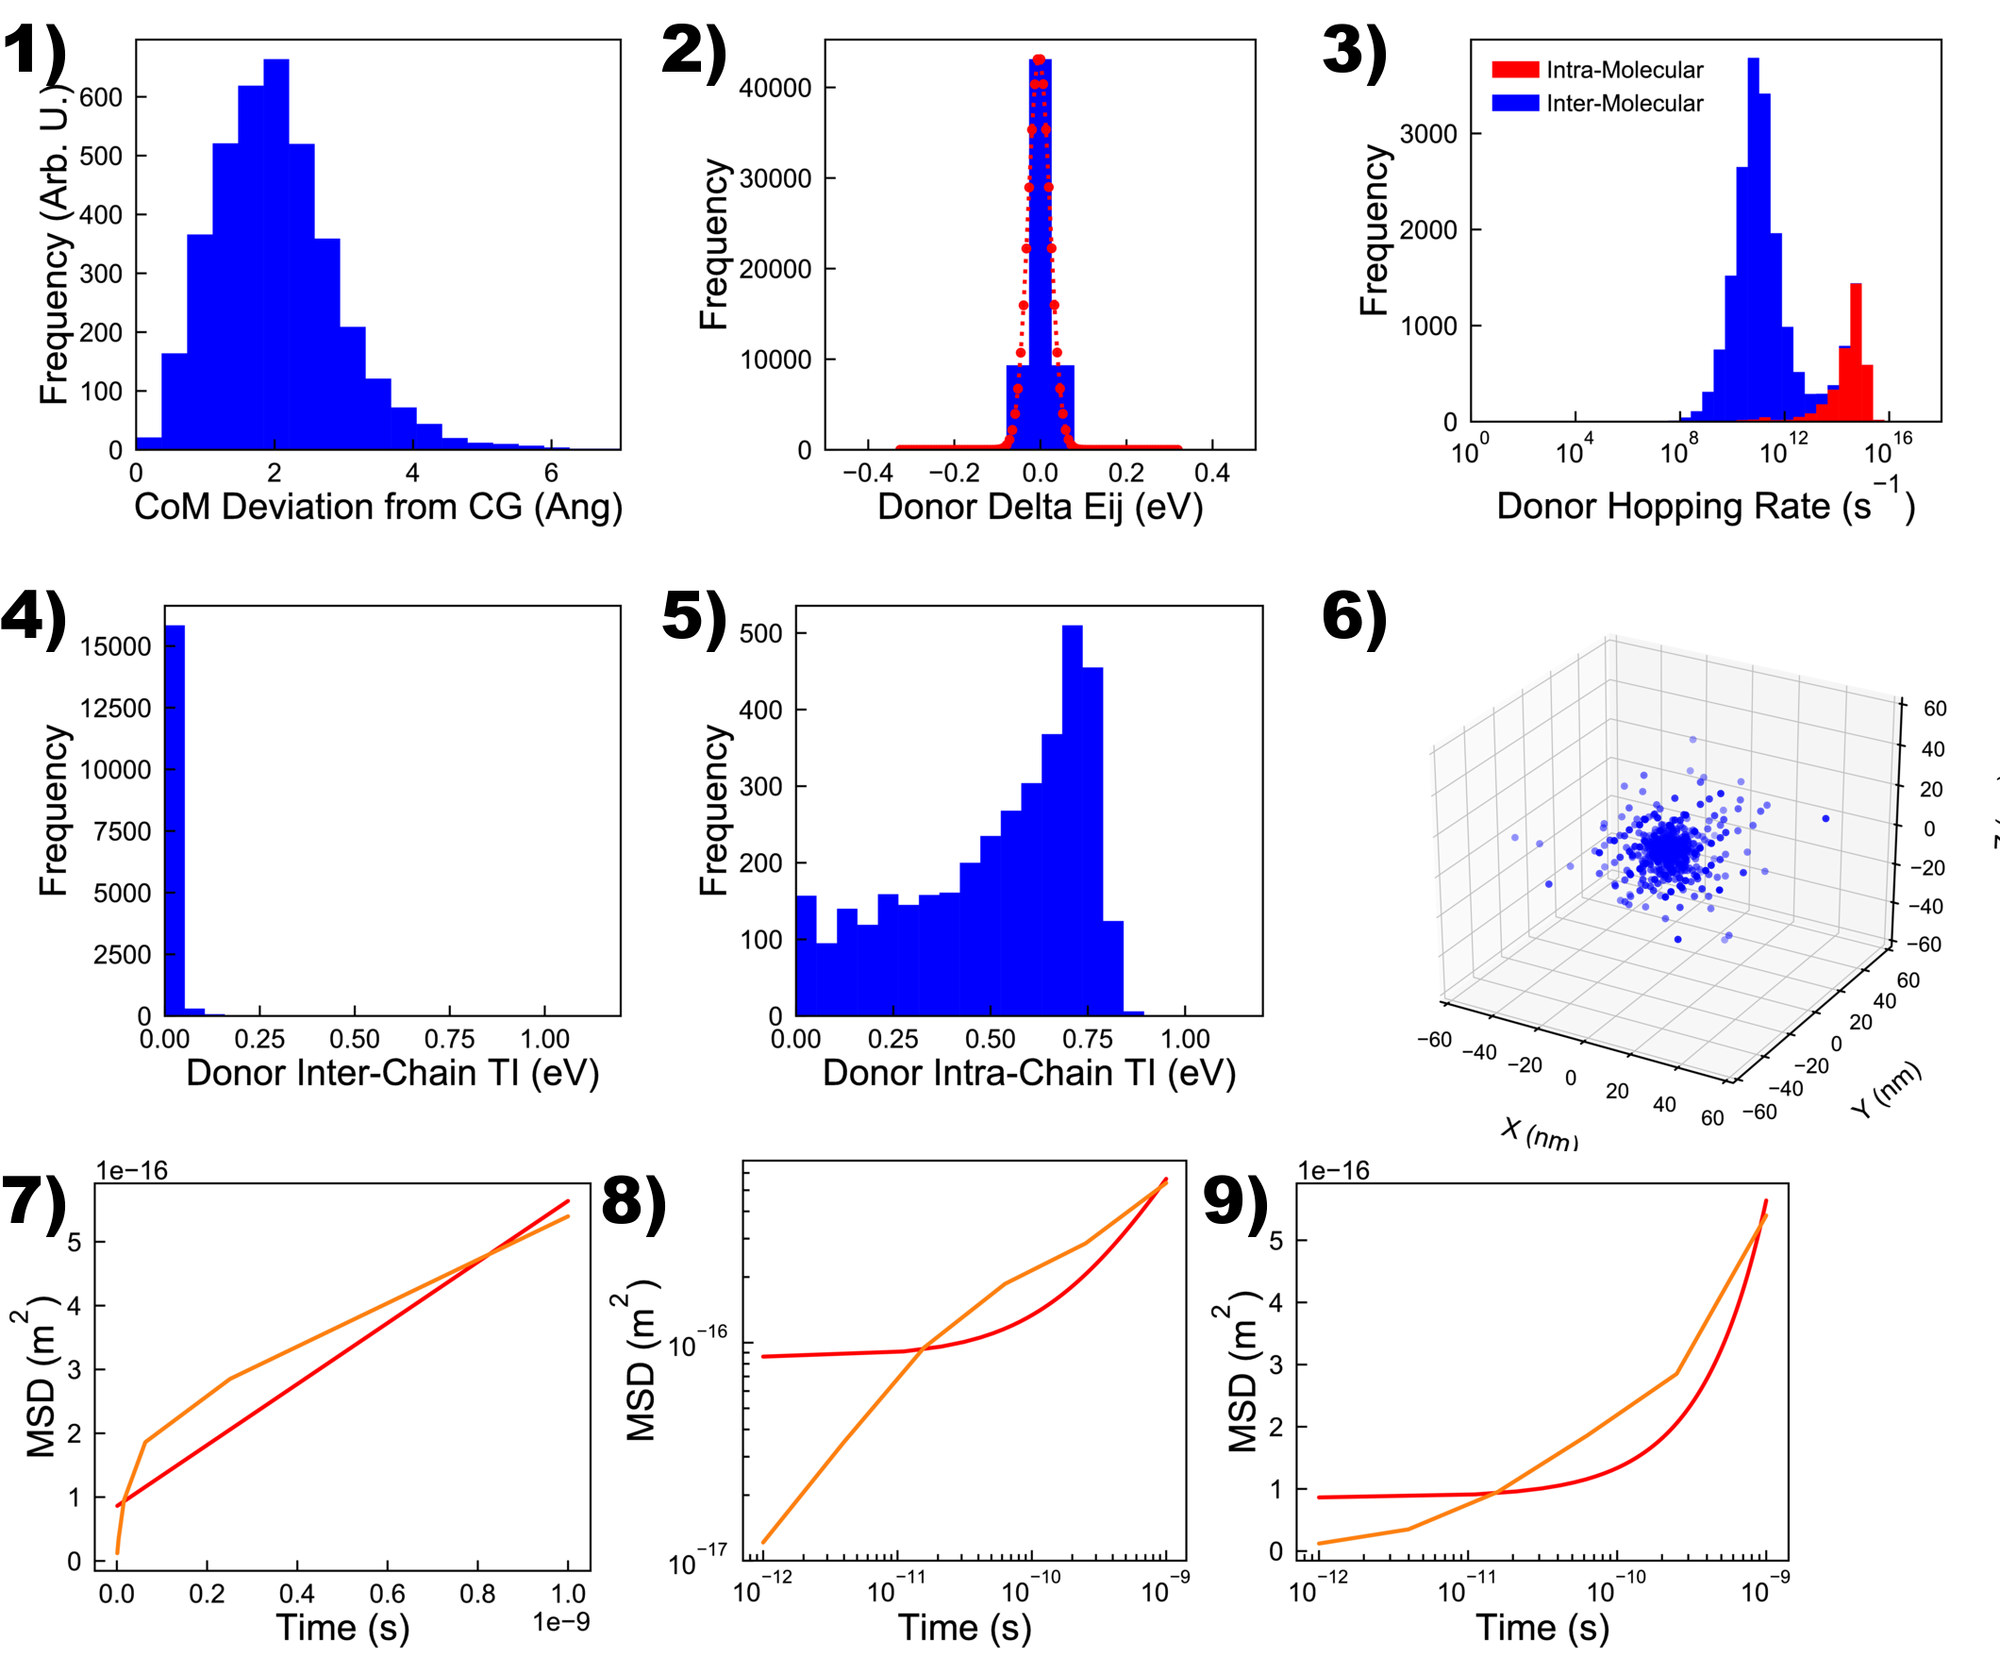
\includegraphics[width=\textwidth]{Figures/T2_25.png}
    \caption{The plots for \textbf{origFG-p1-L15-f0.0-P0.1-T2.25-e0.5}. Plots are as follows: 1) Separation between the CG and fine-grained chromophore CoM, 2) HOMO DoS for chromophores, 3) Hopping rate distribution, 4) Inter-molecular TIs (zeros removed), 5) Intra-molecular TIs (zeros removed), 6) Carrier endpoints after KMC simulation, 7) MSD (Linear scale), 8) MSD (log scale), 9) MSD (semi-log scale)}
	\label{fig:T2.25}
\end{figure}

\begin{figure}[p]\centering
	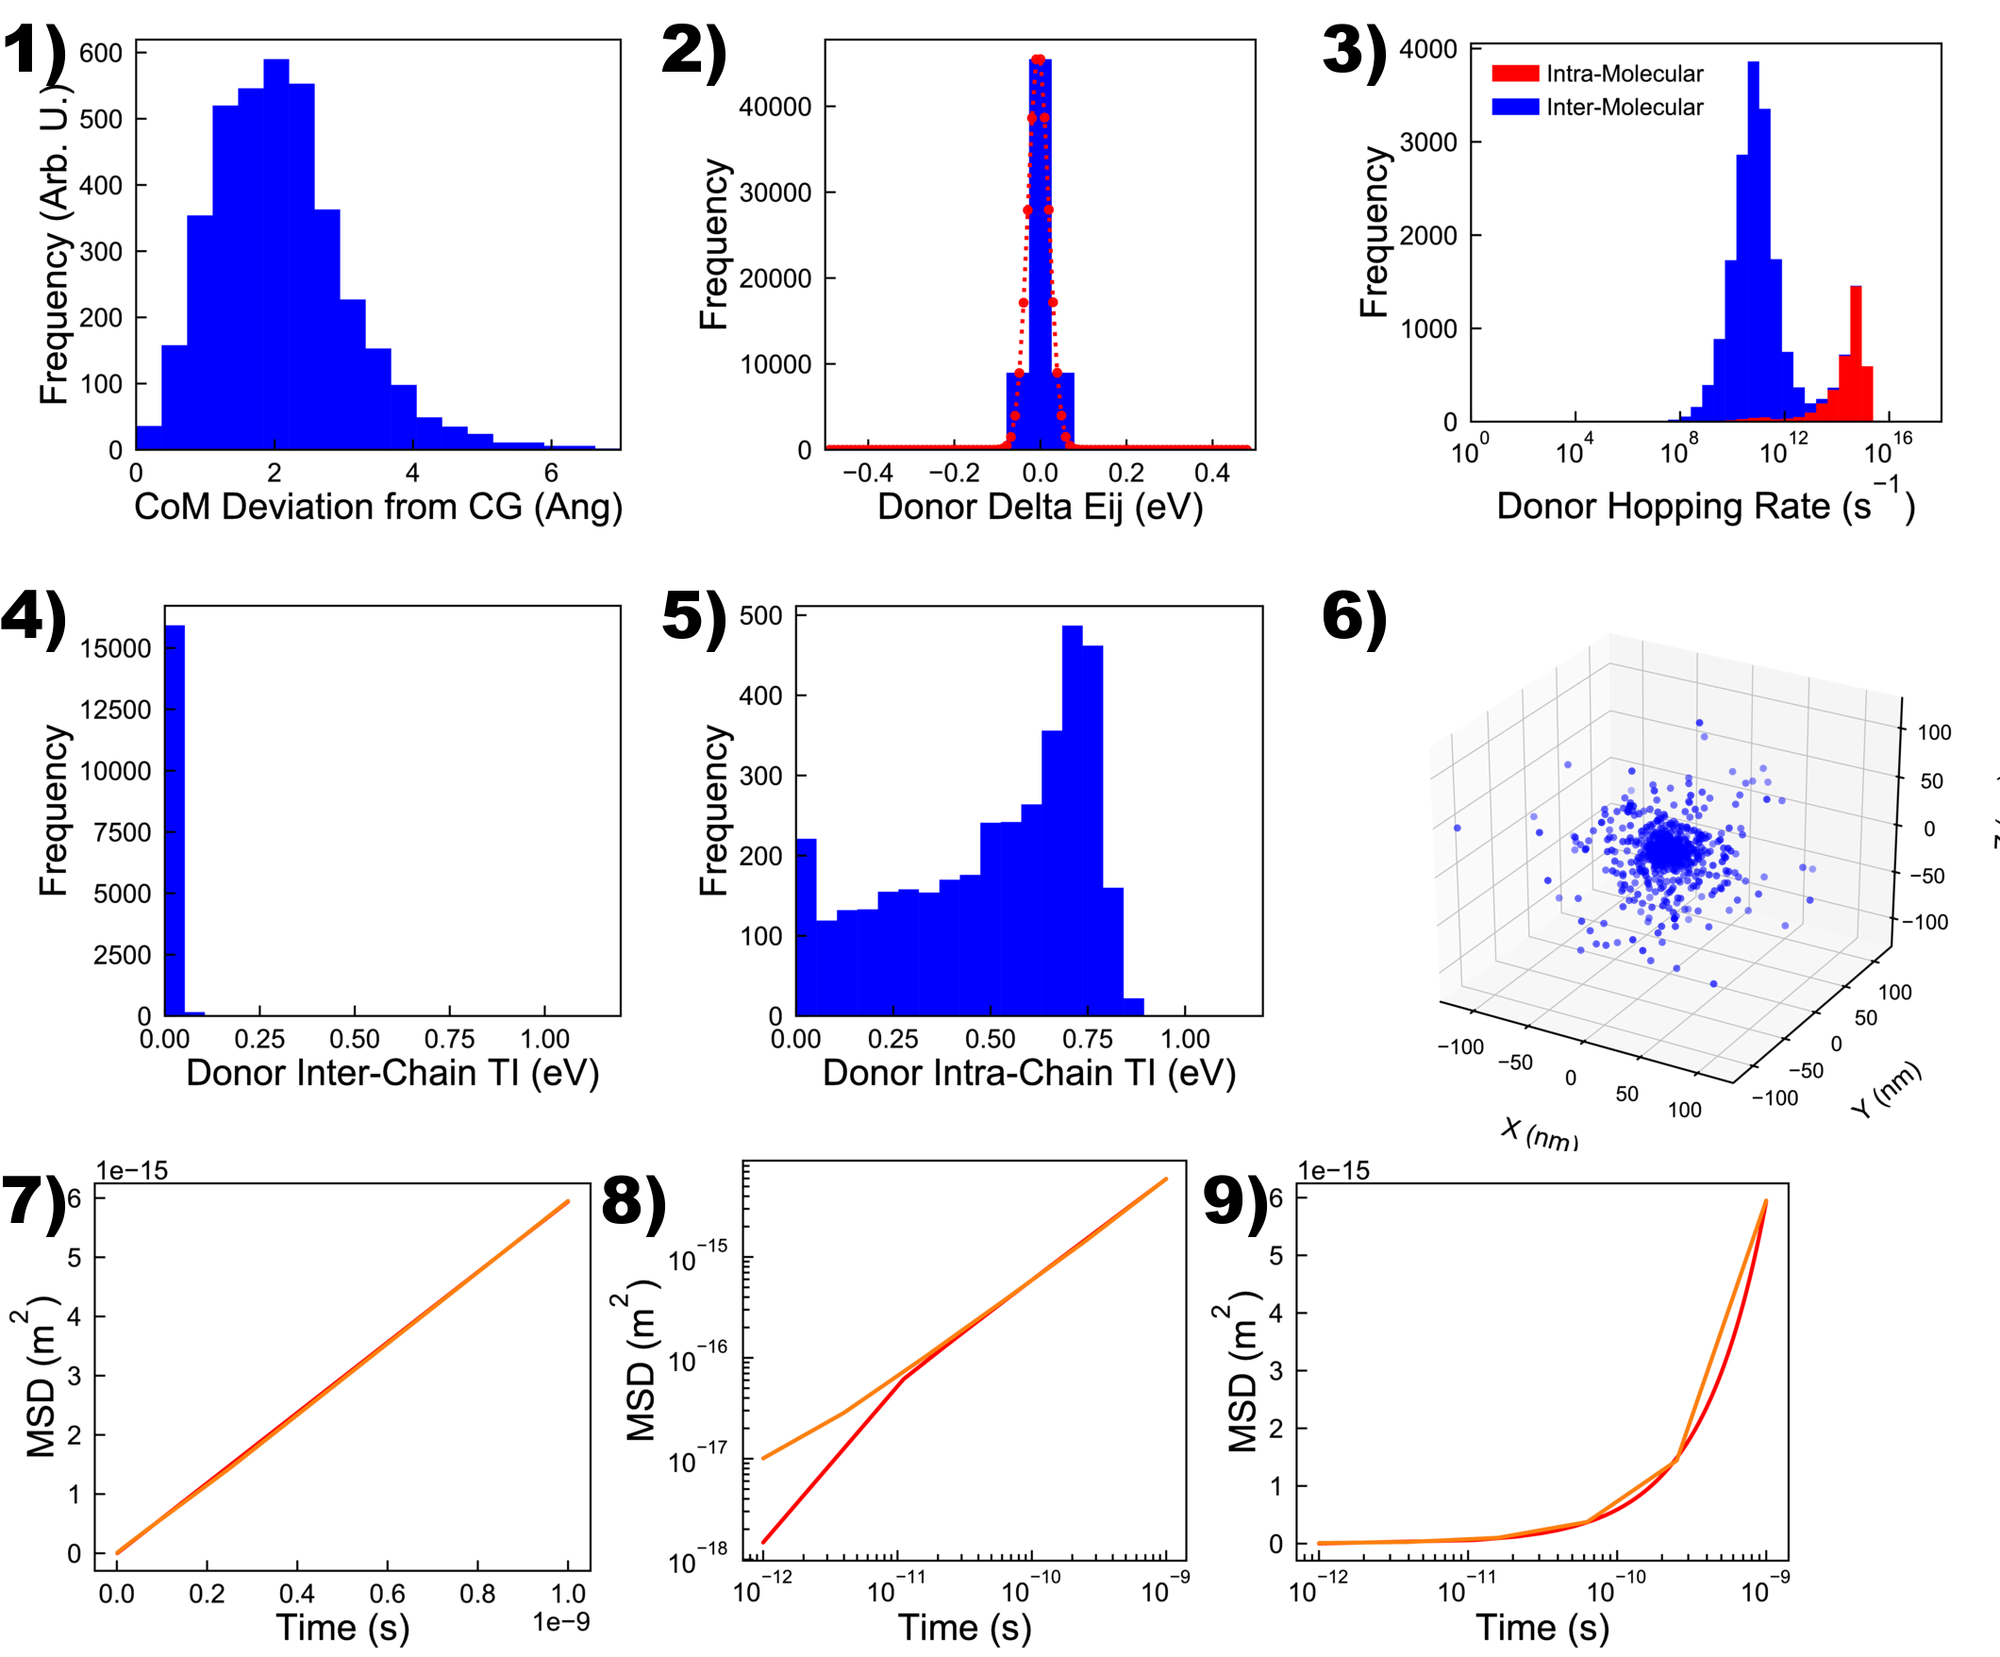
\includegraphics[width=\textwidth]{Figures/T2_5.png}
    \caption{The plots for \textbf{origFG-p1-L15-f0.0-P0.1-T2.5-e0.5}. Plots are as follows: 1) Separation between the CG and fine-grained chromophore CoM, 2) HOMO DoS for chromophores, 3) Hopping rate distribution, 4) Inter-molecular TIs (zeros removed), 5) Intra-molecular TIs (zeros removed), 6) Carrier endpoints after KMC simulation, 7) MSD (Linear scale), 8) MSD (log scale), 9) MSD (semi-log scale)}
	\label{fig:T2.5}
\end{figure}


\clearpage

\subsubsection{Evaluation}


\begin{itemize}
    \item{There are no significant differences between the CoM deviations, hopping rates, DoS, or transfer integrals between the 3 disordered systems.}
    \item{The first difference is that the carriers in the $T = 2.25$ system travel less than half the distance of those in the $T = 2.0$ and $T = 2.5$ systems (anisotropy axes $\sim$50 nm compared to 100).}
    \item{Secondly, the MSD is saturating at longer times, leading to poor fit quality.}
    \item{These two features are linked to the same issue - the network is insufficiently connected to obtain reliable mobility data.}
    \item{This suggestion is born out by the differences between the 3D network plots (Figure \ref{fig:net}) - there is visually significantly more whitespace in the $T = 2.25$ network than for the $T = 2.0$ and (especially) $T = 2.5$ systems.}
    \item{To improve the reliability, averages over several statistically independent frames should be taken and errorbars produced for the mobility values. My hypothesis is that this would produce large error bars and bring the average more into line with the other disordered systems.}
\end{itemize}


\bibliography{refs}
\bibliographystyle{unsrt}


\end{document}
